% This is samplepaper.tex, a sample chapter demonstrating the
% LLNCS macro package for Springer Computer Science proceedings;
% Version 2.20 of 2017/10/04
%
\documentclass[runningheads]{llncs}
%
\usepackage{graphicx}
\usepackage{subcaption}
\usepackage{float}
% Used for displaying a sample figure. If possible, figure files should
% be included in EPS format.
%
% If you use the hyperref package, please uncomment the following line
% to display URLs in blue roman font according to Springer's eBook style:
% \renewcommand\UrlFont{\color{blue}\rmfamily}

\begin{document}
%
\title{Successively Linearized Onboard Reachability\thanks{Supported by organization x.}}
%
%\titlerunning{Abbreviated paper title}
% If the paper title is too long for the running head, you can set
% an abbreviated paper title here
%
\author{Nathan Jewell\inst{1}\orcidID{0000-1111-2222-3333} \and
Houssam Abbas\inst{1}\orcidID{1111-2222-3333-4444} \and
Stanley Baak?\inst{3}\orcidID{2222--3333-4444-5555}}
%
\authorrunning{N. Jewell et al.}
% First names are abbreviated in the running head.
% If there are more than two authors, 'et al.' is used.
%
\institute{Oregon State University, Corvallis OR 97333, USA \and
\email{jewelln@oregonstate.edu}}
%
\maketitle              % typeset the header of the contribution
%
\begin{abstract}
Reachability computations allow for validating safety parameters in various control systems. In this paper we analyze the performance characteristics of successively linearized reachability problems running in realtime. Importantly, we test these running alongside a full suite of autonomous control and localization tools onboard the F1/10 racing platform. A number of runtime modes which utilize single core and multiple core CPU as well as hybridized CPU/GPU were analyzed. In our testing we achieve accurate 10-step reachability as quickly as xxxxx seconds. We find that porting portions of reachability onto the GPU can improve the runtime by xxxx\% and reduces the computational complexity in relation to number of reachability steps.

\keywords{Reachability  \and Safety Analysis \and CUDA }
\end{abstract}
%
%
%
\section{Introduction}
Reachability is the computation and interpretation of possible future agent states at a time or set of times. Given an agent's current state and a range of possible future inputs, a reachability algorithm outputs information about all possible states of the agent at time T in the future. For computational efficiency and practical use, we discuss discrete-time reachability algorithms. In discrete-time reachability, a range of N possible state spaces are generated for N future times. defined by intervals spaced by the discretization time step, dt. Importantly the generated state spaces are minimal overapproximations of possible states as defined by the agent’s dynamical model. This guarantees that any state actually reached at time T is within the overapproximation boundary and can be utilized for safety analysis.

Safety verification is the overarching goal for reachability computations. With highly reliable systems, it is necessary to verify that no error state could be reached. In autonomous vehicles, error states may involve intersections with walls, other cars or people, etc.. By checking the overapproximation of states, it can be determined if the agent is in danger of reaching an error mode in the future. Planned inputs can then be modified to avoid the danger, preventing potentially catastrophic system failure.

We explore a number of different runtime modes for profiling successively linearized reachability computation. These modes are chosen to stress different components of the host system, improve runtime, and demonstrate the effectiveness of real time safety analysis alongside real-world loads.


\section{Setup}


\subsection{Runtime Modes}

\subsubsection{HYLAA} \newline The original hybrid reachability tool [cite].
\vspace*{-5pt}
\subsubsection{Quickzono Single Core} [QZ\_CPU] \newline A simplified subset of HYLAA code with succinct wrappers. 
\vspace*{-5pt}
\subsubsection{Quickzono Multiple Core} [QZ\_MP] \newline Quickzono code with a trivial CPU-based multiprocessing model \newline applied to the projection step. 
\vspace*{-5pt}
\subsubsection{Quickzono GPU Dummy} [QZ\_DUMMY] \newline Quickzono with data copied to and from the GPU but running\newline a dummy kernel on the GPU which does no computation of the projection. 
\vspace*{-5pt}
\subsubsection{Quickzono GPU Hybrid} [QZ\_HYBRID] \newline Hybrid GPU/CPU implementation, with the most taxing\newline part of the projection algorithm moved onto the GPU device. 
\vspace*{-5pt}

\subsection{Offline Profiling}
In offline profiling, reachability is computed as the sole program running on the system. A dedicated testing script executes each of the runtime modes for 200 trials at intervals between 5 to 40 reachability steps. HYLAA is only tested up to 20 steps due to slow performance. The script outputs timing data excluding any one-off setup and configuration code.
\subsection{Online Profiling}
In online profiling, reachability is computed as part of a ROS network running physical control nodes (controller input, motor and servo control, etc..), a GPU based particle filter node for localization, a model predictive control node, and various other supporting nodes. Before beginning the profiling, the vehicle is placed into the test track, localized and configured to autonomously drive the track until profiling is complete. The reachability node is implemented as a wrapper for separate reachability classes (those called by the offline profiler) and records call timings for the same function, executing as quickly as possible. The online profiler is configured to automatically switch between runtimes modes and number of reachability steps. This occurs for the same parameters as in offline profiling except only those configurations executing at least 4hz (<=250ms per trial) are considered. HYLAA is not tested in this profiling due to slow performance.
\subsection{Performance Characteristics}
There are a number of important characteristics needed to describe the performance of a real time embedded algorithm.

Correctness is the assuredness that the outputs are a valid solution to the problem. It is important to know that the algorithm is producing results consistent with the desired output and underlying mathematics. This is especially important for a reachability algorithm which is utilized in safety analysis protocols.

Scalability is how well the algorithm scales with increased problem size. In our case, problem size is dictated by the number of time steps. This corresponds to either or both of an increase in horizon or decrease discretization time step. Horizon (sec) = \#time-step * time-step. It is important to understand how the algorithm scales so intelligent decisions can be made about optimal horizon and precision in real time applications.

Runtime is the time to solve the given problem. Minimizing runtime is a critical component of this research. Running a real time safety algorithm is only effective when there is a low latency between consecutive executions. If this criteria is not met, safety analysis could be out of date when the agent is developing a response, resulting in ineffective performance. In contrast, low latency [runtime] will improve the safety margin of the agent by providing reachability information to the controller which is very up to date with the environment.

Runtime variability is the standard deviation in the runtime. While latency is of primary importance, the consistency of the algorithm runtime is paramount for critical systems. Latency spikes at the wrong time could create dangerous problems for the agent when reacting to unsafe conditions. 

\section{Methods}
\subsection{Collected Data}
Each characteristic has an empirical measure which we can use to analyze it quantitatively. Our offline and online profiling are run separately to evaluate the impact of running the reachability along with localization and control algorithms.

To validate correctness, we used HYLAA model output, assuming that HYLAA is mathematically consistent. Outputs from other runtime modes are compared to the HYLAA output to determine if there are any significant differences. It is not necessary to validate correctness separately for online and offline computation since the same code is executed in each case.

To validate scalability, each runtime model is tested with a range of values for the number of reachability steps which are representative of useful workloads. The number of steps (N) is equal to the ratio between total horizon time in seconds (T) and the discretization time-step (dt). This varying of step values is done for both online and offline modes. However, for online trials, only models capable of running around 200ms per iteration (5hz) are considered.

To test runtime, each combination of runtime mode and steps is evaluated over multiple trials. The recorded runtimes will be the average over 200 trials. This data collection is done for both online and offline testing.

To test runtime variability, the all recorded runtimes from all trials are analyzed. We compute standard deviation in runtime and 95% runtime confidence intervals around the mean assuming normally distributed variation in runtimes. This analysis is performed for both online and offline testing.

Some other values are also collected for the benefit of running analysis. 
What is a trial? One execution of the reachability computation.  


\section{Results}

\begin{figure}[H]
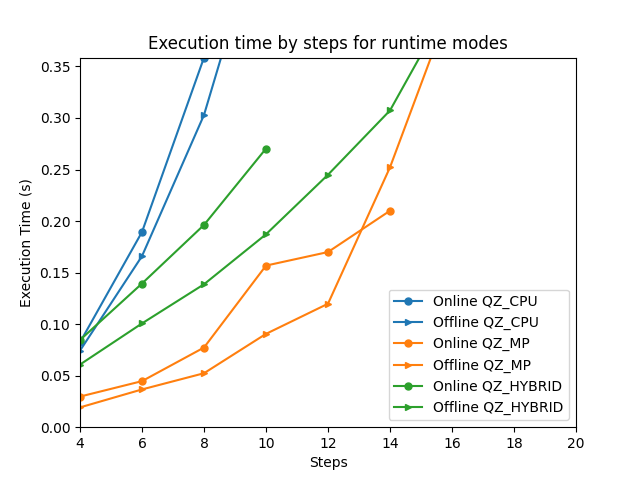
\includegraphics[width=\textwidth]{profiler_out/all_avg_unified.png}
\caption{Average trial execution times for all runtime modes in online and offline configuration.} \label{fig1}
\end{figure}
\begin{figure}[H]
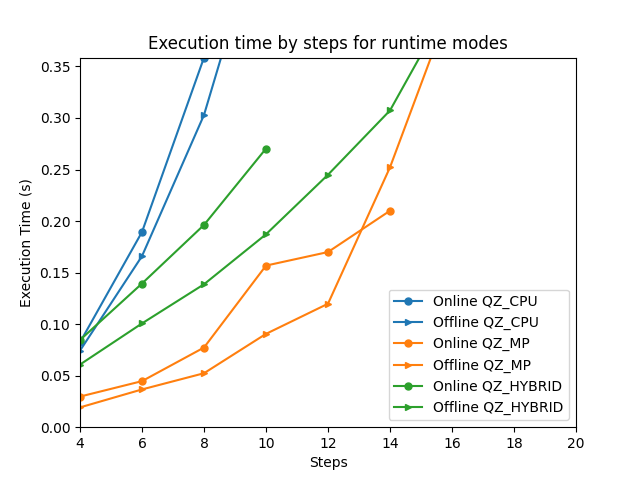
\includegraphics[width=\textwidth]{profiler_out/all_avg_unified.png}
\caption{Average trial execution times for all runtime modes in online and offline configuration.} \label{fig1}
\end{figure}
\begin{figure}[H]
    \subcaptionbox{Detail of the Quickzono GPU Hybrid runtimes with 95\% confidence intervals.\label{CPU_CI}}{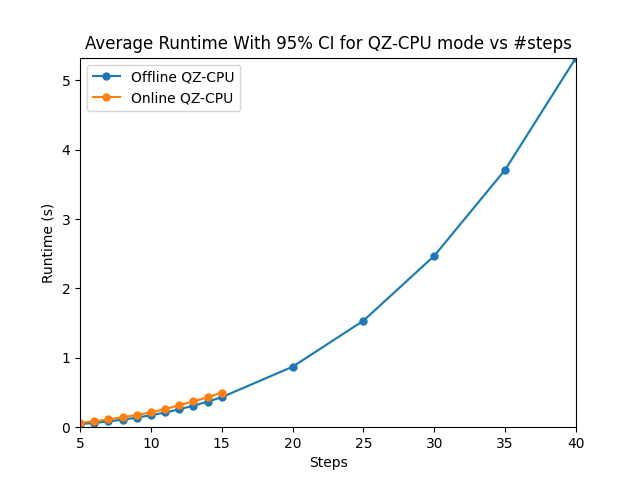
\includegraphics[width=.5\linewidth]{profiler_out/avg_QZ-CPU_CI.png} }
    \subcaptionbox{Detail of the Quickzono Single Core runtimes with 95\% confidence intervals.\label{MP_CI}}{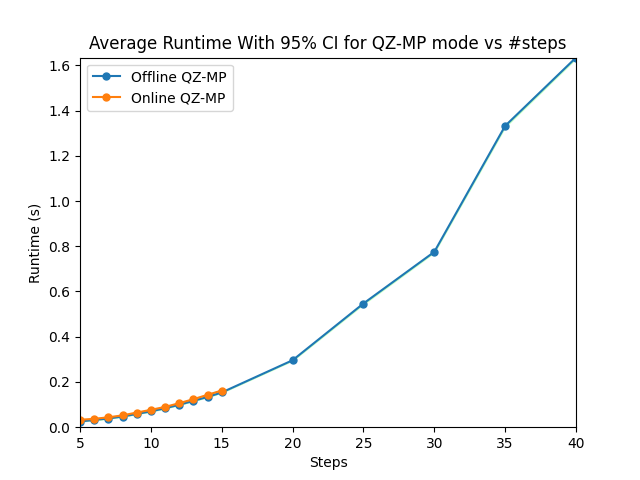
\includegraphics[width=.5\linewidth]{profiler_out/avg_QZ-MP_CI.png} }
\begin{subfigure}{\linewidth}
    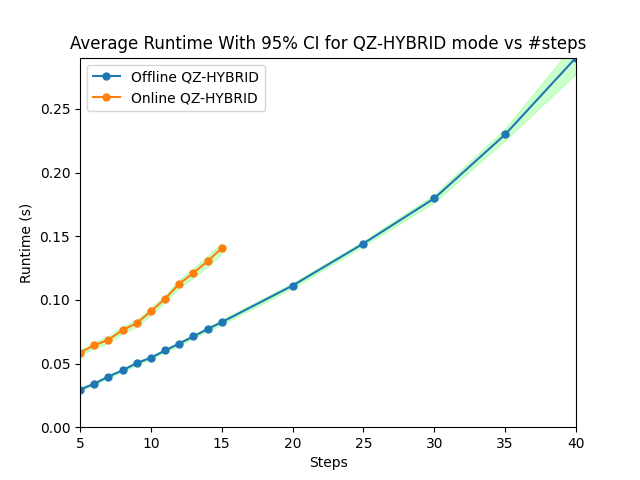
\includegraphics[width=.5\linewidth]{profiler_out/avg_QZ-HYBRID_CI.png}
    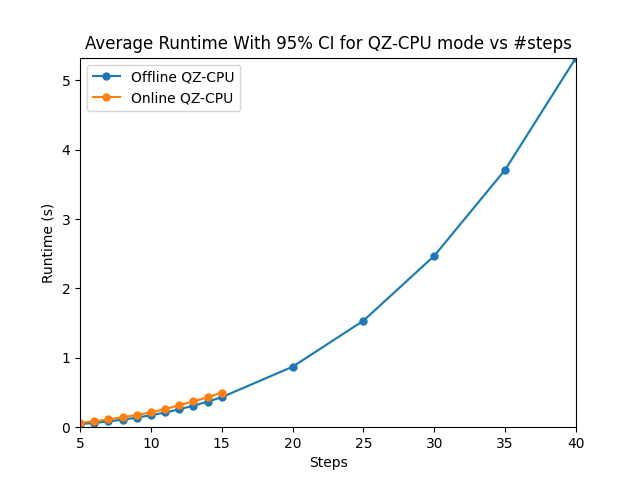
\includegraphics[width=.5\linewidth]{profiler_out/avg_QZ-CPU_CI.png} \hfill

\end{subfigure}

\end{figure}

\section{Discussion}

%
% ---- Bibliography ----
%
% BibTeX users should specify bibliography style 'splncs04'.
% References will then be sorted and formatted in the correct style.
%
% \bibliographystyle{splncs04}
% \bibliography{mybibliography}
%
\begin{thebibliography}{8}


\bibitem{ref_hylaa}
HYLAA Author, F., Author, S.: Title of a proceedings paper. In: Editor,
F., Editor, S. (eds.) CONFERENCE 2016, LNCS, vol. 9999, pp. 1--13.
Springer, Heidelberg (2016). \doi{10.10007/1234567890}

\bibitem{ref_oder}
ODER Author, F., Author, S., Author, T.: Book title. 2nd edn. Publisher,
Location (1999)

\end{thebibliography}
\end{document}
